\documentclass[12pt]{article}
\usepackage[ruled, vlined]{algorithm2e}
\usepackage{amsmath, amsfonts, amssymb, mathrsfs}
\usepackage{caption}
\usepackage{dcolumn}
\usepackage{filemod}
\usepackage{floatrow}
\usepackage{gensymb}
\usepackage{graphicx}
\usepackage{hyperref}
\usepackage{natbib}
\usepackage{setspace}
\usepackage{subcaption}
\usepackage{verbatim}
\usepackage{makecell}

\oddsidemargin=0.25in
\evensidemargin=0.25in
\textwidth=7in
\textheight=8.75in
\topmargin=-.5in
\addtolength{\oddsidemargin}{-.5in}
\addtolength{\evensidemargin}{-.5in}
\footskip=0.5in

\begin{document}

\title{Bayesian Statistical Inversion for High-Dimensional Computer Model
Output and Spatially Distributed Counts}
\author{Steven D. Barnett\thanks{Corresponding author
\href{mailto:sdbarnett@vt.edu}{\tt sdbarnett@vt.edu}, Department of
Statistics, Virginia Tech} \and Robert B. Gramacy\thanks{Department of
Statistics, Virginia Tech} \and Lauren J. Beesley\thanks{Statistical Sciences
Group, Los Alamos National Laboratory} \and Dave Osthus\footnotemark[3] \and
Yifan Huang\thanks{ Nuclear and Particle Physics, AstroPhysics and Cosmology,
Los Alamos National Laboratory} \and Fan Guo\footnotemark[4] \and Eric J.
Zirnstein\thanks{ Department of Astrophysical Sciences, Princeton University}
\and Daniel B. Reisenfeld\thanks{Space Science and Applications Group, Los
Alamos National Laboratory}}
\date{}

\maketitle

%\vspace{-0.5cm}

\begin{abstract}
Data collected by the Interstellar Boundary Explorer (IBEX) satellite,
recording heliospheric energetic neutral atoms (ENAs), exhibit a phenomena
that have caused space scientists to revise hypotheses about the physical
processes, and computer simulations under those models, in play at the
boundary of our solar system.  Evaluating the fit of these computer models
involves tuning their parameters to observational data from IBEX. This would
be a classic (Bayesian) inverse problem if not for three challenges: (1) the
computer simulations are slow, limiting the size of campaigns of runs; so (2)
surrogate modeling is essential but outputs are high-resolution images
thwarting conventional methods; and (3) IBEX observations are counts, whereas
most inverse problem techniques assume Gaussian field data. To fill that gap
we propose a novel approach to Bayesian inverse problems coupling a Poisson
response with a sparse Gaussian process surrogate using the Vecchia
approximation.  We demonstrate the capibilities of our proposed framework,
which compare favorably to alternatives, through multiple simulated
examples in terms of recovering ``true'' computer model parameters and accurate
out-of-sample prediction. We then apply this new technology to IBEX satellite
data and associated computer models developed at Los Alamos National Lab.

\bigskip
\noindent \textbf{Key words:} Gaussian process, surrogate modeling,
Poisson, calibration, heliospheric science, IBEX, Vecchia approximation
\end{abstract}

\doublespacing % no double spacing for arXiv

%%%%%%%%%%%%%%%%%%%%%%%%%%%%%%%%%%%%%%%%%%%%%%%%%%%%%%%%%%%%%%%%%%%%%%%%%%%%%%%

\section{Introduction}
\label{sec:intro}

%% IBEX
%% - Talk about the satellite
%% - Explain the mission
%% - Introduce the idea of a computer model
%% - Explain desire to understand the distribution of parameters
The National Aeronautics and Space Administration (NASA) launched the
Interstellar Boundary Explorer (IBEX) satellite in 2008 as part of their Small
Explorer program \citep{mccomas2009aIBEX} to deepen our understanding of the
heliosphere. The heliosphere is the bubble formed by the solar wind that
encompasses our solar system and acts as a barrier to interstellar space. Of
particular interest is the behavior at the edge of the heliosphere, known as
the heliopause. Here, highly energized hydrogen ions that make up the solar
wind interact with neutral atoms, occasionally undergo electro exchange, and
become neutral themselves. These energetic neutral atoms (ENAs) are unaffected
by magnetic fields and therefore travel in a straight line.

Some ENAs eventually make their way to Earth and can be detected by an
instrument on the IBEX satellite called the IBEX-Hi ENA imager
\citep{funsten2009IBEXHiENA}. This apparatus records the energy level and
approximate location of origin for each ENA that enters the detector. IBEX's
raw collected data consist of ENA counts and exposure times for each area of
the sky at which the satellite points, providing sufficient information to
estimate the rate at which these particles are created throughout the
heliopause. An example of this estimated surface or image, referred to by
space scientists as a \textit{sky map}, can be found in the left panel of Fig.
\ref{f:fig1}. Sky maps are integral to better understand the heliosphere's
creation and evolution.

\begin{figure}[ht!]
\centering
\includegraphics[scale=0.75,trim=0 0 65 0,clip=TRUE]{ibex_real1.pdf}
\includegraphics[scale=0.75,trim=35 0 65 0,clip=TRUE]{sim1.pdf}
\includegraphics[scale=0.75,trim=35 0 20 0,clip=TRUE]{sim2.pdf}
\caption{Observed ENA rate detected by the
IBEX satellite (left) and output from two IBEX  simuations under
different parameter settings (middle, right).
\label{f:fig1}}
\end{figure}

One can think of the heliosphere as a ``boat'' moving through interstellar
space. At the outset of IBEX's mission, scientists expected to see an elevated
rate of ENAs being generated at the front (nose) and back (tail), much like
the turbulent interaction with water at a boat's bow and stern. And indeed,
that belief was validated by IBEX data. These predicted regions of raised ENA
rates are known as \textit{globally distributed flux}, or GDF. At the nose and
tail there are an increased number of collisions between hydrogen ions and
neutral particles in the interstellar medium.

However, in a completely unanticipated finding, IBEX also recorded a thin
string of higher rates of ENAs \citep{fuselier2009IBEXribbon} wrapping around
the heliosphere. Scientists now refer to this phenomenom as the
\textit{ribbon}. This unique feature of a sky map is clearly visible in Fig.
\ref{f:fig1}. Since this discovery, space scientists have proposed several
theories attempting to describe the physical process that generates the ribbon
\citep{mccomas2014ibex, zirnstein2018role, zirnstein2019strong,
zirnstein2021dependence}.

Computer models encapsulating competing theories have been built which
generate high-resolution (i.e, a high-dimensional response) synthetic sky maps
(middle and right panels of Figure \ref{f:fig1}). These simulations are
extremely sophisticated and involve many complex and expensive operations,
such as the solving of partial differential equations. Consequently, executing
a single run of the computer model at a specified set of model parameters can
take thousands of core hours.  This severely limits the number of unique 
runs generating simulated sky in various conditions. 

Our work here focuses on two, publicly accessible computer models: a GDF
model proposed by \citet{zirnstein2021heliosheath}; and a ribbon-only model
developed by \citet{zirnsteinGDFsims2015}. These simulators take inputs that
can be varied to modify the shape and intensity of both ribbon and GDF. The
ribbon-only model relies on two parameters, \textit{parallel mean free path}
and \textit{ratio}, while the GDF model takes \textit{kappa} and
\textit{pickup ions (PUI) cooling index} as inputs. Dialing in good settings
for these input parameters, in light of observed ENA counts from IBEX, is
instrumental in furthering theory development and validation.

Space scientists at Los Alamos National Lab (LANL) wish to solve this ``parameter
tuning'' exercise as a Bayesian inverse problem
\citep{kaipio2011bayesian,stuart2010inverse,knapik2011bayesian}, obtaining a
posterior distribution over likely settings.  However, the exposure and count data
IBEX provides, along with computer simulated rates, present some unique challenges:
1) computationally intensive models limiting simulation, necessitating surrogate
modeling; 2) high-dimensional model output (simulated sky maps, each containing
tens of thousands of pixels), thwarting conventional surrogate modeling
techniques; 3) a non-Gaussian field response (Poisson counts).  It is worth noting
that Bayesian posterior sampling, say via Markov chain Monte Carlo (MCMC),
compounds computational bottlenecks (2). We propose a framework for Bayesian
inverse problems that utilizes the Vecchia approximation
\citep{katzfuss2021general,scaledvecchiakatzfuss2022} with a Gaussian process (GP)
surrogate or emulator for high dimensional computer simulations, and couple that
with a Poisson observational model to furnish posterior samples of unknown
parameters to these models given observed data.

Methods exist separately, in the literature, to address needs in each of the
aforementioned situations 1)--3), but we are not aware of anything in the
intersection. Table \ref{tab:prev_work} summarizes the features of the IBEX inverse
problem and reviews the necessary capabilities, alongside recent papers offering
partial solutions.  References provided are representative.  We acknowledge that
there are, in most cases, several works that may fit the bill.  Each row in the table
may be summarized as follows.

\begin{table}[ht!]
\centering
\renewcommand{\arraystretch}{1.5}
\begin{tabular}{|l|c|c|c|c|}
\hline
& Bayesian & \makecell{Non-\\Gaussian} & \makecell{Large-Scale \\ Simulation \\ Output} & \makecell{High-Dim \\ Response} \\
\hline
Our Contribution & \checkmark & \checkmark & \checkmark & \checkmark \\
\hline
\citet{kennedyohagan2001} & \checkmark & & & \\
\hline
\citet{higdoncalib2008} & \checkmark & & & \checkmark \\
\hline
\citet{gramacy2015calibrating} & & & \checkmark & \\
\hline
\citet{grosskopfcountcalib2020} & \checkmark & \checkmark & & \\
\hline
\end{tabular}
\caption{Check marks indicate that functionality exists within the cited paper and/or
accompanying software. To save space, only one citation is listed for each
row.}
\label{tab:prev_work}
\end{table}

\citet{kennedyohagan2001} offer the canonical computer model calibration
framework, which provides a fully Bayesian approach to estimate the posterior
distribution of calibration parameters and improve prediction at new,
unobserved field locations. However, their methodology is limited to Gaussian
field observations and small, simulator output. \citet{higdoncalib2008} and
SEPIA \citep{gattiker2020lanl}, its more recent incarnation, also employ
Bayesian methods while accounting for computer model output that is
functional. But SEPIA is somewhat rigid, does not scale well with added model
runs, and requires the user to specify a number of basis functions to
represent the simulator response. \citet{gramacy2015calibrating} consider
computer model calibration with large-scale output from a computer experiment,
necessitating an approximation. But their implementation is not Bayesian and
the scale of simulator data is still orders of magnitude less than IBEX.
\citet{grosskopfcountcalib2020} provide an extension of the Kennedy \& O'Hagan
(hereafter referred to as KOH) framework to non-Gaussian data that maintains a
Bayesian approach. But they are limited to small amounts of computer model
data and do not consider higher dimensional responses. In contrast, our
approach checks all the boxes to achieve the goal of IBEX space scientists and
therefore applies to a wider class of problems than previous work.

Our integrated framework for Bayesian inverse problems overcomes these obstacles
together in an all-in-one solution, as illustrated in the top row of Table
\ref{tab:prev_work}. We adopt the approach of generalized computer model calibration,
adapting to IBEX's count data with a Poisson likelihood and employing MCMC to garner
posterior samples of model parameters, which determine the underlying mean of our
Poisson model, given observed data. These samples allow us to estimate the full joint
posterior distribution of the unknown parameters. We access predicted ENA rates
through a GP surrogate or emulator fit to a limited set of expensive,
high-dimensional IBEX computer simulations to more thoroughly explore the domain of
possible sky maps that serves as the basis for the observed ENA counts. As previously
stated, MCMC exacerbates the computational burden of making surrogate predictions,
necessitating not only a sparse GP surrogate, but one that can swiftly generate
repeated sky map proposals at each MCMC iteration. We find the Vecchia approximation
to be extremely effective in this regard. Lastly, we propose a more intuitive
technique to modeling high-dimensional vectors, treating each pixel representing an
ENA rate as a scalar response of interest. This differs from previous approaches to
functional computer model output, but enables us to leverage recent advances in
sparse GP surrogate modeling. Additionally, using this strategy efficiently scales
both to increased dimensionality of the response and to larger sizes of training
sets.

%% OUTLINE
%% - Review Bayesian Inverse Problems, GP Surrogates, SEPIA
%% - Introduce our framework
%% - Explain use of Vecchia approximation
%% - Demonstrate on simulated data
%% - Apply to real IBEX data
Our paper is laid out as follows. First, Section \ref{sec:review} reviews
methods that form the foundation for our work, namely Bayesian Inverse Problems
and Gaussian process surrogate models. We also give a brief description of the
methodology and implementation behind SEPIA, which could be classified as the
current ``status quo'' in Bayesian Inverse Problems for high-dimensional
computer model output. In Section \ref{sec:gen_bayes_inv} we introduce our
framework for solving the inverse problem in non-Gaussian contexts. Section
\ref{sec:vecchia} describes our use of the Vecchia approximation to stretch the
capacity of a GP surrogate beyond small simulator training runs. In Section
\ref{sec:synth_data}, we illustrate the effectiveness of our framework in
discovering the true, underlying model parameters on synthetic data. We then
return to our motivating application and apply our methods to the raw IBEX
satellite data in Section \ref{sec:ibex_real}. To conclude, we discuss any
extensions and future work in Section \ref{sec:discuss}. Our implementation may
be found at \url{https://github.com/lanl/IBEX_Calibration} along with code
reproducing all included examples.

%%%%%%%%%%%%%%%%%%%%%%%%%%%%%%%%%%%%%%%%%%%%%%%%%%%%%%%%%%%%%%%%%%%%%%%%%%%%%%%

%%%%%%%%%%%%%%%%%%%%%%%%%%%%%%%%%%%%%%%%%%%%%%%%%%%%%%%%%%%%%%%%%%%%%%%%%%%%%%%

% SECTION 2: Review:
\section{Bayesian inverse problems}
\label{sec:review}

We study IBEX through the lens of observational data $Y^F$ ($F$ for field
measurement) and a computer implementation of a physical model $m(u, X)$,
where parameters $u$ are unknown and $X$ represents the spatial locations
where the simulation output is evaluated.  These may be the locations $X^F$
that correspond to field measurements $Y^F$, or a grid of predictive locations
supporting high resolution visuals.  Given prior information about $u$, we
want to know which $u$'s lead to realizations of $m(\cdot, \cdot)$ that could
explain $Y^F$, i.e., the posterior for $u \mid Y^F$. 

This is a classic Bayesian inverse problem
\citep{kaipio2011bayesian,stuart2010inverse,knapik2011bayesian}. Eq.~\ref{eq:inv_bayes_mod} 
provides the typical hierarchical model used in this
setting.
\begin{align}
Y^F &\sim \mathcal{N}_{n_F}\!\left(\mu\!\left(X^F\right),
\Sigma\!\left(X^F\right)\right) \nonumber  \\
\mu(X) &= m(u, X) \label{eq:inv_bayes_mod} \\
\Sigma(X) &\sim \pi\left(\Sigma\right) & \mbox{e.g.,} \quad \Sigma^{-1} & \sim \mathrm{Wishart}((\rho V)^{-1}, \rho)
\nonumber \\
u &\sim \pi(u) & \mbox{e.g.,} \quad u &\sim \mathrm{Unif}[0,1]^p \nonumber
\end{align}
One big difference with Bayesian inverse problems, as opposed to ordinary
Bayesian inference, is that the parameters $\mu(X^F)$ and $\Sigma(X^F)$
defining the distribution of $Y^F$ are not of direct interest. Rather, we are
interested in settings $u$ that define
$\mu(X)$ and $\Sigma(X)$ through $m(u, X)$.  For example, two different
settings of $u$ were used in the IBEX simulator to generate the center and
right panels of Figure \ref{f:fig1}. Colors indicate output $\mu(X)$ values on
a dense grid $X$ of longitudes and latitudes. We are interested in learning
which $u$ are likely to have generated the recorded $Y^F$ values in the left
panel, observed at locations where the IBEX satellite was pointed ($X^F$) to
collect particles.

To help fix ideas, consider the simpler example introduced in the left panel
of Figure \ref{f:toy_calib}. Red stars indicate noisy field measurements,
$Y^F$, observed in replicate as $y_i \stackrel{\mathrm{iid}} \sim
\mathcal{N}(m(u^\star, x_i), \sigma^2)$ for a ``true'' unknown $u^\star =
(u_1^\star, u_2^\star)^\top$ and uniform $x_i \in X^F$.  In this simple
example, the computer model $m(\cdot, \cdot)$ was used to generate the data.
In practice, the model represents a caricature using known or best-guess
physics. Each light gray line is a realization of $m(\cdot, \cdot)$ for a
different $u$ on a fine grid of spatial locations $X$. The bold-black-dashed
line is $m(u^\star, X)$ provided as a reference.

\begin{figure}[ht!]
\centering
\includegraphics[scale=0.55,trim=20 0 30 0,clip=TRUE]{logit1_obs.pdf}
\includegraphics[scale=0.55,trim=59 0 30 0,clip=TRUE]{logit1_est.pdf}
\includegraphics[scale=0.55,trim=16 0 30 0,clip=TRUE]{logit1_post_draws.pdf}
\caption{A simple inverse problem. Field observations and a small sample of
computer model runs (left), model evaluations at posterior draws and mean
(middle), and posterior distribution of model parameters (right).
\label{f:toy_calib}}
\end{figure}

The middle panel of the figure shows runs of our virtual model evaluated at posterior
draws of $u$ obtained under Metropolis sampling using a multivariate
normal likelihood whose mean $\mu(X^F)=m(u^{(t)}, X^F)$ and whose covariance $\Sigma(X^F) \sim \sigma^2
\mathbb{I}$, where $\sigma^2$ is marginalized out under a reference prior
$\pi(\sigma^2) \propto 1/\sigma^2$. Although we display these runs on a
high-resolution grid $X$, the sampler only uses evaluations of $m(u^{(t)}, X^F)$ in
likelihood evaluations. The posterior samples of $u$ thus obtained are shown
in the right panel of the figure.  In this toy example, it is evident that the
Metropolis sampler successfully concentrates posterior mass around the true
value of $u$.

The literature on Bayesian inverse problems involves methods that work
predominantly in this way, particularly as regards a Gaussian likelihood. We
aim to provide a method that achieves the same goal, but for unknown parameters
$u$ that underlie observed IBEX satellite data (left panel of Figure
\ref{f:fig1}), whose observations are counts under variable exposure. Our first
contribution, which is albeit rather straightforward, is to depart from that
literature by perusing a Poisson likelihood.

%------------------------------------------------------------------------------
%% SECTION 2.1 - Generalized Bayesian inverse problems
\subsection{Generalized Bayesian inverse problems}
\label{sec:gen_bayes_inv}
%------------------------------------------------------------------------------

Our IBEX observations $Y^F$ are counts under exposure $e(X^F)$, which is at odds
with the canonical Gaussian likelihood in the Bayesian inverse problem setup
introduced earlier. We wish to model a count $y \sim \mathrm{Pois}(\lambda, e)$
where $f(y|\lambda, e) = \frac{(\lambda e)^y \mathrm{exp}\{-\lambda e\}}{y!}$.
We thereby extend Eq.~(\ref{eq:inv_bayes_mod}) as follows:
\begin{align}
Y^F &\sim \mathrm{Pois}(\lambda(X^F), e(X^F)) & \lambda(X) &= m(u, X) \nonumber
\label{eq:pois_inv_bayes_mod} \\ u &\sim \pi(u) & \mbox{e.g.,} \quad u &\sim \mathrm{Unif}[0,1]^p,
\end{align}
where $e(X^F)$ represents the duration (in seconds) the satellite points at
specific locations in the sky. $\lambda(X^F)$ denotes the rate at which ENA
particles are generated for rows (latitude/longitude pairs) in $X^F$. Sampling
from the posterior could proceed via Metroplis as in Algorithm \ref{alg:gibbs}.
For the IBEX field data, we evaluate a Poisson likelihood given an exposure
time for each observation and a mean surface determined by a simulator
$m(\cdot,\cdot)$ at proposed values of $u$, although we believe it would be
straightforward to accommodate other observational models.
\begin{algorithm}[ht]
\DontPrintSemicolon
Initialize $u^{(0)}$. \\
Set $\lambda(X^F)^{(0)} = m(u^{(0)}, X^F)$. \\
Compute and store $\mathcal{L}(Y^F|\lambda(X^F)^{(0)}, e(X^F)) =
\prod_{i=1}^{n_F} f(y_i|\lambda_i, e_i)$, \\
\For{$t = 1, \dots, T$}{
  Propose new model parameters: $u^{(t)} \sim q(u^{(t)} \mid u^{(t-1)})$, \\
  \vspace{0.2em}
  Evaluate simulator at field locations and $u^{(t)}$: $\lambda(X^F)^{(t)} = m(u^{(t)}, X^F)$,
  \\
  \vspace{0.2em}
  Calculate and save $\mathcal{L}(Y^F|\lambda(X^F)^{(t)}, e(X^F)) =
  \prod_{i=1}^{n_F} f(y_i|\lambda_i(X^F)^{(t)}, e_i)$, \\
  \vspace{0.2em}
  Compute the acceptance ratio: $\alpha = \frac{\mathcal{L}\left(Y^F \mid
  \lambda(X^F)^{(t)}, e(X^F)\right) \pi\left(u^{(t)}\right) q\left(u^{(t-1)}
  \mid u^{(t)}\right)}{\mathcal{L}\left(Y^F \mid \lambda(X^F)^{(t-1)},
  e(X^F)\right) \pi\left(u^{(t-1)}\right) q\left(u^{(t)} \mid
  u^{(t-1)}\right)}$, \\ Accept or reject $u^{(t)}$. }
\caption{MCMC (Metropolis-within-Gibbs) for Poisson Bayesian inverse problems}
\label{alg:gibbs}
\end{algorithm}

Using Algorithm \ref{alg:gibbs}, we can build on the toy problem we introduced
in Figure \ref{f:toy_calib} and align it more closely with the IBEX data.
Instead of observing a mean process $\mu(X^F)$ with random, Gaussian noise,
suppose we are given counts, drawn from a Poisson process with $\lambda(X^F) =
m(u^*, X^F)$, as shown in the left panel of Figure \ref{f:toy_calib_pois}.
Computer model runs $m(\cdot,\cdot) = \lambda(X)$ produce different mean
surfaces given unique values of $u = (u_1, u_2)$. Observed counts are shown as
red stars. Red circles indicate the sum of all counts at one input location
(i.e, a single row of $X^F$) divided by the sum of their corresponding exposure
times $e(\cdot)$. These points are the actual data we receive. Results from
running Algorithm \ref{alg:gibbs} are shown in the middle and right panels of
Figure \ref{f:toy_calib_pois}. Similar to the results in Figure
\ref{f:toy_calib}, it is clear that the sampler searches a broad swath of the
model input space but hones in on the region where the true parameter value
lies.
\begin{figure}[ht!]
\centering
\includegraphics[scale=0.55,trim=20 0 30 0,clip=TRUE]{logit1_pois_obs.pdf}
\includegraphics[scale=0.55,trim=59 0 30 0,clip=TRUE]{logit1_pois_est.pdf}
\includegraphics[scale=0.55,trim=16 0 30 0,clip=TRUE]{logit1_pois_post_draws.pdf}
\caption{An inverse problem for a Poisson process. Counts observed in the field
and a sample of computer model runs (left), model evaluations at posterior
draws and mean (middle), and posterior distribution of model parameters
(right).
\label{f:toy_calib_pois}}
\end{figure}

In each of these examples we have made the assumption that we have unlimited
access to simulator runs (i.e, for each proposed combination of model
parameters, we can quickly get a response from the computer simulation). But
that is rarely the case, presenting another challenge to the typical Bayesian
inverse problem apparatus. For instance, each run of the IBEX model $m(\cdot,
\cdot)$ is a Herculean effort, requiring hundreds or thousands of core hours on
a supercomputer.  That simply cannot be embedded in a Metropolis sampler
requiring thousands of iterations to convergence.  While it's rather
conventional to deploy a surrogate model \citep[e.g.][]{gramacy2020surrogates}
in this setting, trained on a design of space-filling $u$-values, doing so
effectively is challenged by the dimension of $X^F$.  We considered multiple
surrogate models developed to accomodate such scenarios (e.g. GPs via inducing
points \citep{banerjee2008gaussian}, local approximate GPs
\citep{gramacy2014lagp}), but found them unable to manage the scale of the IBEX
data. Herein lies our main methodological contribution, using a modern sparse
approach to surrogate modeling in a (Poisson) Bayesian inverse problem setting.
The remainder of this section outlines the standard surrogate modeling toolkit,
as a jumping-off point toward explaining both our main comparative (Section
\ref{sec:gp_approx}) and our main methodological contribution.

%------------------------------------------------------------------------------
%% SECTION 2.2 - Gaussian Process Surrogates for Computer Experiments:
\subsection{Gaussian process surrogates for computer experiments}
\label{sec:gp_surr}
%------------------------------------------------------------------------------

Evaluating the likelihood $Y_F$ in Algorithm \ref{alg:gibbs} may proceed via
surrogate when {\em in situ} evaluation directly on $m(\cdot, \cdot)$ is too
slow. Suppose we have a vector of observations $Y^M$ at input locations $X^M$
from a campaign of runs of $m(\cdot, \cdot)$ that may or may not coincide with
settings in $X^F$. We prefer a small design of space-filling $u$-values ($U$),
paired via Cartesian product with $X^F$ from the field experiment or a
predictive grid $X$, e.g., $X^M = X \otimes U$, depending on the situation.
Two such runs, i.e., for two rows $u^\top \in U$ and a dense grid $X$, are shown
in Figure \ref{f:fig1}.

Given a corpus of runs $(Y^M, X^M)$, a surrogate synthesizes this information
in order to extend it to new inputs.  Many surrogates for computer
simulations are based on Gaussian processes
\citep[e.g.,][]{rasmussen2003gaussian}, where modeling boils down to
specifying a multivariate normal (MVN) for all responses.  This way,
prediction is simply a matter of MVN conditioning rules, or {\em kriging}
\citep{matheron1963principles}, to derive the distribution of unknown
(testing) output given known (training) values. Specifically, let $Y^M
\sim \mathcal{N}_{n_M}(\mu(X^M), \Sigma(X^M))$, where $\mathcal{N}_{n_M}$
indicates an $n_M$-variate MVN. Then, predicting at a new location $x$ (think
proposed $u$-value and paired row in $X^F$) follows $Y(x) \mid Y(X^M) \sim
\mathcal{N}(\hat{\mu}(x), \hat{\sigma}^2(x))$, where
\begin{align}
\hat{\mu}(x) &= \mu(x) + \Sigma(x, X^M) \Sigma(X^M)^{-1} (Y^M - \mu(X^M)) \label{eq:mvn_eq}\\
\hat{\sigma}^2(x) &= \Sigma(x, x) - \Sigma(x, X^M) \Sigma(X^M)^{-1} \Sigma(X^M, x). \nonumber
\end{align}
Although a generic mean function is specified in Eq.~(\ref{eq:mvn_eq}), it is
common to set $\mu(\cdot)=0$ assuming pre-centered responses. In this zero-mean
context, all the action takes place in the covariance function $\Sigma(x, x')$,
which is usually specified as inversely poportional to distances between inputs
$x$ and $x'$. We use a form known as the separable Mat\'ern kernel
\citep{stein1999interpolation} in our work, a conventional choice, parameterized
by lengthscales $\theta$ and scale $\tau^2$. For details, see \citep[][Chapter
5]{gramacy2020surrogates}. GPs provide a flexible, nonparametric regression
tool. In addition to enjoying canonical status as surrogates for computer
simulation experiments, they are utilized in geospatial statistics
\citep{cressie2011statistics}, time series \citep{roberts2013gaussian}, and
optimization \citep{jones1998efficient}.

GP surrogates are extremely effective. To illustrate, recall Figures
\ref{f:toy_calib} and \ref{f:toy_calib_pois} in Section \ref{sec:gen_bayes_inv},
where limited samples of computer model evaluations ($n < 50$) are shown. For
these toy examples, we ``assumed'' we had unlimited access to the simulator. In
reality, we fit a GP surrogate to the model runs in the left panels. Therefore,
``model runs'' at posterior draws of $u$ in the center panels are not in fact
evaluations of the model, but predictions from a fitted GP surrogate. Even so,
the Metropolis sampler used those accurate (and fast) predictions to
successfully recover the true model parameters $u^*$.

One downside to working with MVNs whose dimension grows with the dimension of
the data they are trained on, $n_M$, is that building $n_M \times n_M$ matrices,
and inverting (or otherwise decomposing) them, e.g., for Eq.~(\ref{eq:mvn_eq})
requires storage and computation that is quadratic and cubic in $n_M$,
respectively.  This limits $n_M$ to a few thousand at most in a Bayesian MCMC
setting, necessitating approximations for GPs that curb this prohibitive cost.
With the 1d example in Figure \ref{f:toy_calib_pois}, we have $n_M=20 \times
40$, combining $X$ and $U$, which is manageable. But for IBEX, the simulated sky
maps like those in the middle and right panels of Figure \ref{f:fig1} are in 2d
(under the hood the output is in spherical coordinates $x$, $y$, and $z$) and
results in $>16{,}000$ locations (or pixels) for each $u$-value. Combine that
with $n=66$ unique $u$-values and our response vector will have greater than one
million elements. Even if we used a smaller LHS space-filling design of size
$n=15$ over the model parameters, the response vector would still consist of
over 200,000 points. In that case, a GP could not be fit and provide predictions
in a reasonable amount of time, prompting the next topic.

%------------------------------------------------------------------------------
%% SECTION 2.3 - Approximations
\subsection{Approximations}
\label{sec:gp_approx}
%------------------------------------------------------------------------------

Most of our modeling effort in this paper involves circumventing the $O(n_M^3)$
computational bottleneck associated with GPs. The prevalence of methods
addressing this issue has grown significantly in the past decade as increased
access to computing resources leads to problems with larger and larger training
datasets. These methods include, but are not limited to, fixed-rank kriging
\citep{cressie2008fixed}, inducing points \citep{banerjee2008gaussian},
compactly supported kernels \citep{kaufman2011efficient}, divide-and-conquer
\citep{gramacy2015local}, and nearest neighbors \citep{datta2016hierarchical,
wu2022variational}. Most of these are general enough to be used in a variety of
different fields and applications. However, there is a method tailor-made for
our Bayesian inverse problem setting when the likelihood (for $Y_F$) is
Gaussian.

Specifically in the context of (Gaussian) inverse problems,
\citet{higdoncalib2008} faced computational bottlenecks much like the IBEX
simulator: expensive simulations limiting runs and high dimensional output in
the form of images, shape description, time series, etc. Even with today's
computing resources, it would be prohibitive to fit a GP surrogate model on such
large data. \citeauthor{higdoncalib2008}'s key insight involved treating $X^F$
(or gridded $X$) -- i.e., the fixed reference set that a simulator realization
is evaluated on for each candidate parameter $u$ -- as a feature of {\em
output}, rather than conventionally as an input. As a result, model and field
data share the same set of measurement locations, that is, $X = X^F$. In this
way, $X^M$ remains small, including only the unique combinations of unknown
parameters $u$.

Then, rather than keep track of all of those outputs $Y^M$, indexed over $X^F$
or $X$, dimensionality may be drammatically reduced via principal components
analysis (PCA). Specifically, they proposed representing the vector output of
a simulator model $m(\cdot,\cdot)$ as the sum of $n_k$ basis functions $k_1,
k_2, \ldots , k_{n_k}$, each scaled by a corresponding weight $w_i(u)$.
\begin{equation}
m(u, X) \approx \sum_{i=1}^{n_k}  k_i \cdot w_i (u),
\quad \mbox{ where } \quad w_i(u) \sim \mathcal{N}( 0, \Sigma_{w_i}) 
 \quad \mbox{and} \quad n_k \ll n_X.
\label{eq:higdon_pca}
\end{equation}
Weights $w_i(u)$ are each modeled as realizations of a zero-mean GP. By not
directly modeling the high-dimensional response $m(\cdot,\cdot)$ and it's
associated dense grid $X$, requesite decompositions $\Sigma_{w_i}$ avoids the
cubic bottleneck in computation when scaling to large $n$ and can be completed
in a reasonable amount of time.

While clever, this is one of those easy-to-say hard-to-do situations. The
implementation is complex both mathematically, and in code.  We are aware of
only one library implemenation, originally written in {\sf MATLAB} and now
deployed in {\sf Python} \citep{gattiker2020lanl},  We found it difficult to
approporiate that setup for our own use in a Poisson likelihood context.
Addtionally, restricting the simulated and field data to work on the same
reference grid was not possible with IBEX's orbital data locations (Figure
\ref{f:fig1}).

Fortunately, GP approximation has come a long way in the last
twenty or years. \citeauthor{higdoncalib2008} specifically lamented not having
access to such technology, necessitating a more complex approach. It is no
longer necessary to play the trick of moving a reference grid to the output
space.  A GP (approximation) may model $Y^M$ via all inputs $X^F$ and $U$ via
$X^M$, as we shall demonstrate next.  The result is at once more modern, faster,
and better compartmentalized for use in novel contexts, such as our own.

%%%%%%%%%%%%%%%%%%%%%%%%%%%%%%%%%%%%%%%%%%%%%%%%%%%%%%%%%%%%%%%%%%%%%%%%%%%%%%%

%%%%%%%%%%%%%%%%%%%%%%%%%%%%%%%%%%%%%%%%%%%%%%%%%%%%%%%%%%%%%%%%%%%%%%%%%%%%%%%

%------------------------------------------------------------------------------
%% SECTION 3 - Vecchia Approximated GPs for IBEX Simulations
\section{Vecchia Approximated GPs for IBEX Simulations}
\label{sec:vecchia}
%------------------------------------------------------------------------------

In 1988, \citeauthor{vecchia1988estimation} proposed an approximation for
evaluating a multivariate normal density. The Vecchia approximation, say in the
context of GP modeling with the likelihood for $Y^M$ (i.e. $\mathcal{L}(Y^M)$),
relies on the ability to write any joint probability as a cascade of univariate
conditionals, which for GPs are Gaussian (\ref{eq:mvn_eq}).
\begin{align}
\mathcal{L}(Y^M)&=\prod_{i=1}^{n_M} \mathcal{L}(Y^M_i \mid Y^M_{g(i)})
\hspace{0.3em} \mbox{ where } g(1)=\emptyset \hspace{0.3em} \mbox{ and }
g(i)=\{1, 2, \ldots, i-1\} \nonumber \\
&\approx \prod_{i=1}^{n_M}\mathcal{L}(Y^M_i \mid Y^M_{h(i)}) \hspace{0.3em} \mbox{
where } h(i) \subset \{1, 2, \ldots, i-1\} \hspace{0.3em} \mbox{ and } |h(i)| \ll n_M
\label{eq:vecchia}
\end{align}

\citeauthor{vecchia1988estimation}'s critical observation was that one could
approximate this function by reducing the size of the conditioning set $g(i)$
to a much smaller size $m$, as specified by the user. This induces sparsity in
the precision matrix (e.g. $\Sigma(X^M)^{-1})$ from Eq.~\ref{eq:mvn_eq},
potentially dramatically speeding up the evaluation of the likelihood for large
values of $n_M$. \citet{katzfuss2021general} recently made this approximation
popular by working out its representation in matrix form and furnishing
automatic $h(i)$ via nearest neighbor and code, allowing for broad use in a
variety of different fields where GPs are employed, particularly spatial
statistics and computer experiments
\citep{guinness2018permutation,katzfuss2020vecchia,katzfuss2021general,zhang2022multi,sauer2023vecchia}.

The Vecchia approximation takes an operation of order $O(n_M^3)$ down to $O(n_M
m^3)$, motivating small values of $m$. Logically, as the size of $h(i)$
decreases, the evaluation of the likelihood speeds up, but the quality of the
approximation is reduced. On the flip side, as one increases $m$, execution
time grows, but the degree of accuracy improves. This continues until $n=m-1$,
when the likelihood is no longer an approximation. For the IBEX simulator data,
we find a value of $m=25$ to be more than sufficient.

Several implementations of the Vecchia approximation exist, but we employ one
that has risen to the top in terms of predictive performance and computational
thriftiness in the context of computer experiments, that is, the Scaled Vecchia
approximation introduced by \citet{scaledvecchiakatzfuss2022}. We refer you to
their manuscript for a more in-depth explanation of their work, but the primary
draw for using it as a surrogate for the IBEX simulator is the open source
implementation and packaging that leverages modern sparse matrix libraries and
parallel processing. Code that that we directly rely on is readily accessible at
\url{https://github.com/katzfuss-group/scaledVecchia}.

%------------------------------------------------------------------------------
%% SECTION 3.1 - Surrogate Sky Maps
\subsection{Surrogate Sky Maps}
\label{sec:surr_skymaps}
%------------------------------------------------------------------------------

Figure \ref{f:ibex_vecchia} illustrates examples of conditioning sets created
by the Scaled Vecchia approximation in the context of IBEX and its associated
simulator. (We will circle back to the inverse problem and the data collected by
the satellite in Section \ref{sec:synth_data}). Neighborhoods of size $m \in
\{25,50,75,100\}$ are generated for a particular simulator observation $Y_i^M$
(denoted by a red star) from the IBEX computer model. It's difficult to
visualize in higher dimensions, so we break the input space down into separate
2d plots, one for grid space (latitude/longitude) and one for model parameter
space ($u$). But to be clear, points of the same shape and color in both plots
are elements of the same overall conditioning set. For each conditioning set
$h_j(i)$, all points from sets where $m < m_j$ are also included in $h_j(i)$.
That is, green circles from the neighborhood with $m=25$ would also be part of
the conditioning set with blue squares ($m=50$). For reference, we've overlaid
the points in grid space on a grayed-out simulated sky map corresponding with
the observation of interest. Note that more points are concentrated near the
reference point in latitude and longitude, whereas the neighborhood is more
spread out over the unknown model parameters. This behavior is present in all
conditioning sets in IBEX. Therefore, observations condition on information in
close proximity in grid space, but potentially distant in $u$-space.
Furthermore, as $m$ grows, additional points in grid space are mostly farther
away than those already included, but we don't observe the same trend in
$u$-space.

\begin{figure}[ht!]
\centering
\includegraphics[scale=0.5, trim=5 0 30 0,clip=TRUE]{ibex_nbr_latlon.pdf}
\includegraphics[scale=0.5, trim=5 0 30 0,clip=TRUE]{ibex_nbr_params.pdf}
\caption{Conditioning sets $h(i)$ in a multivariate normal likelihood
(Eq.~\ref{eq:vecchia}) for a single observation $Y_i^M$ using the Scaled
Vecchia approximation. The left panel visualizes neighborhoods in grid space
(i.e. $X$ or $X^F$). Model parameter ($u$) space is displayed in the right
panel with jitter added.
\label{f:ibex_vecchia}}
\end{figure}

We begin evaluation of Scaled Vecchia's performance on the IBEX simulator with
a visual assessment. Scientists at LANL have provided us with 66 unique model
runs, each producing an image of 16,200 points, or pixels. Figure
\ref{f:ibex_sim_surr} shows four of the actual simulation outputs (corner
panels displayed with thin, solid borders). A Scaled Vecchia surrogate is fit
to all 66 simulated runs. Then, we predict the output for five unobserved
combinations of the model parameters that fall in between the actual runs
shown. These are depicted in the cross of Figure \ref{f:ibex_sim_surr}, those
panels with thicker, dashed borders. To the naked eye, these predictive
surfaces appear to have been generated by the computer model itself. Moving
left to right, or top to bottom, the surfaces change gradually and as one would
expect. Next we show empirically that our surrogate fit is extremely accurate
and outperforms competitors.

\begin{figure}[ht!]
\centering
\includegraphics[scale=0.5,trim=5 38 65 0,clip=TRUE]{ibex_sim_pmfp_1500_0.005.pdf}
\includegraphics[scale=0.5,trim=35 38 65 0,clip=TRUE]{ibex_sim_pmfp_1625_0.005.pdf}
\includegraphics[scale=0.5,trim=35 38 65 0,clip=TRUE]{ibex_sim_pmfp_1750_0.005.pdf}
\includegraphics[scale=0.5,trim=5 38 65 0,clip=TRUE]{ibex_sim_pmfp_1500_0.0075.pdf}
\includegraphics[scale=0.5,trim=35 38 65 0,clip=TRUE]{ibex_sim_pmfp_1625_0.0075.pdf}
\includegraphics[scale=0.5,trim=35 38 65 0,clip=TRUE]{ibex_sim_pmfp_1750_0.0075.pdf}
\includegraphics[scale=0.5,trim=5 0 65 0,clip=TRUE]{ibex_sim_pmfp_1500_0.01.pdf}
\includegraphics[scale=0.5,trim=35 0 65 0,clip=TRUE]{ibex_sim_pmfp_1625_0.01.pdf}
\includegraphics[scale=0.5,trim=35 0 65 0,clip=TRUE]{ibex_sim_pmfp_1750_0.01.pdf}
\caption{Actual and predicted outputs from the IBEX \textit{sky map} computer
model. Corner panels represent the response for four unique combinations of
model inputs. Panels on the cross with bold, dashed borders are predictions at
unobserved input combinations from a GP surrogate fit to $n=66$ runs of the
computer model. Model parameter settings for the predictive panels fall between
the four actual simulator runs shown.
\label{f:ibex_sim_surr}}
\end{figure}

%------------------------------------------------------------------------------
%% SECTION 3.2 - Empirical Comparison
\subsection{Empirical Comparison}
\label{sec:emp_comp}
%------------------------------------------------------------------------------

To benchmark our surrogate, we conduct experiments to gauge predictive accuracy
via root mean squared error (RMSE), uncertainty quantification via continuous
ranked probability score \citep[CRPS;][]{gneiting2007strictly}, and
computational efficiency via time. We carry out the same experiment for three
competitors: {\sf R} packages {\sf laGP} \citep{gramacy2014lagp} with defaults
and {\sf deepgp} \citep{deepGP} with 1000 MCMC iterations and {\sf vecchia =
TRUE}, and the current ``status-quo'' SEPIA \citep{gattiker2020lanl} with $n_k
= 3$, implemented in {\sf Python}.

Figure \ref{f:ibex_surr_metrics} displays the accuracy results of a simple
hold-one-out bakeoff, with time coming next. For each iteration of the
experiment, we fit a Scaled Vecchia GP surrogate on 65 of the $n=66$ model runs
available. Then, we predict at the held out model parameter. For now, just pay
attention to the boxplots on the left-hand side of each panel. We'll come back
to the others in a moment. It is obvious that the Scaled Vecchia approximation
outperforms {\sf laGP} and {\sf deepgp} in both RMSE and CRPS. SEPIA performed
similarly to our Scaled Vecchia approximation, illustrating why it has had such
staying power over the past two decades. As a practitioner, it appears to be a
toss-up between these two methods for which to use. But that's not the entire
story.

\begin{figure}[ht!]
\centering
\includegraphics[scale=0.45, trim=0 0 0 0,clip=TRUE]{ibex_surr_rmse.pdf}
\includegraphics[scale=0.45, trim=0 0 0 0,clip=TRUE]{ibex_surr_crps.pdf}
\caption{Metrics on the IBEX simulator experiment. Smaller is better for both
RMSE and CRPS.
\label{f:ibex_surr_metrics}}
\end{figure}

Figures \ref{f:ibex_surr_timing_dim}-\ref{f:ibex_surr_timing_size} summarize
compute times in a similar experiment but varying data size. Two factors exist
that contribute to a computational bottleneck: the dimension of the simulator
response (the main focus of our work), and the number of runs of the computer
model available for training. To test scaling dimension, we vary the
dimensionality of the response from 200 to 20,000, while keeping the number of
runs constant. For the two methods that are best equipped for large dimensions
(Scaled Vecchia and SEPIA), we attempt to stretch their capacity by cranking up
the length of the response vector from 20-75K by steps of 5K. At each dimension
size, we ran five Monte Carlo iterations for each method and recorded the
average elapsed time.

\begin{figure}[ht!]
\centering
\includegraphics[scale=0.57, trim=0 0 0 0, clip=TRUE]{ibex_surr_fit_times.pdf}
\includegraphics[scale=0.57, trim=0 0 0 0, clip=TRUE]{ibex_surr_pred_times.pdf}
\includegraphics[scale=0.57, trim=0 0 0 0, clip=TRUE]{ibex_surr_total_times.pdf}
\caption{Timing metrics on the IBEX simulator experiment.
\label{f:ibex_surr_timing_dim}}
\end{figure}

It is plainly visible from Figure \ref{f:ibex_surr_timing_dim} that Scaled
Vecchia and SEPIA are both well-suited for increasing dimensionality in the
response. Our {\sf deepgp} competitor needs to decompose an $n_M \times n_M$
matrix at each MCMC iteration, which causes it's cost to quickly grow as
dimensionality expands, even aided by the Vecchia approximation. While {\sf
laGP} does better, it is unable to keep pace at a certain point, likely due to
the need to fit a mounting number of local GPs separately for each testing
location. Reducing the neighborhood size for {\sf laGP} could help reduce
computation, but would further degrade it's performance. The comparison between
Scaled Vecchia and SEPIA is more nuanced. In the right panel of Figure
\ref{f:ibex_surr_timing_dim}, we see that for a fixed value of $m$, Scaled
Vecchia's runtime increases linearly with expanded dimensionality, as
consistent with claims made by \citet{katzfuss2021general}. For a fixed number
of principal components, SEPIA's execution time increases only slightly as
dimension expands, showcasing it's utility. However, for response dimension
less than 75K, Scaled Vecchia with $m=25$ still executes faster. And that may
be the largest value of $m$ we need. The boxplots on the right-hand side of
each panel in Figure \ref{f:ibex_surr_metrics} show that increasing $m$ or
$n_k$ doesn't significantly improve performance. It must also be pointed out
that the IBEX simulator surface is not particularly complex over the model
parameters, allowing SEPIA to perform well with a low value of $n_k$. That may
not be the case in other situations, requiring more principal components and by
extension a heavier computational load.

Figure \ref{f:ibex_surr_timing_size} displays timing results from changing the
size of the training dataset (i.e, the number of simulator runs $n$). SEPIA was
specifically built for computer experiments with high-dimensional output. While
it clearly performs well in these situations, it's also fairly inflexible to
other contexts, such as a large number of simulation runs. Scaled Vecchia does
not face this hurdle, as it treats both high-dimensional output and large-scale
univariate datasets similarly, as a univariate response. Our experiment is set
up similar to the previous one, but we keep the dimensionality of the response
at 10K while sliding the number of simulator runs from 10 to 100. Again, all
method are run over five MC iterations for each value of $n$. For the higher
performing methods, we push the campaign size up further ($n=2500$).

\begin{figure}[ht!]
\centering
\includegraphics[scale=0.57, trim=0 0 0 0, clip=TRUE]{ibex_surr_fit_times_ns.pdf}
\includegraphics[scale=0.57, trim=0 0 0 0, clip=TRUE]{ibex_surr_pred_times_ns.pdf}
\includegraphics[scale=0.57, trim=0 0 0 0, clip=TRUE]{ibex_surr_total_times_ns.pdf}
\caption{Timing metrics on the IBEX simulator experiment.
\label{f:ibex_surr_timing_size}}
\end{figure}

It's no surprise that {\sf deepgp} once again lags in run time. Even a modest
sized set of runs takes well over an hour to fit and needs almost 10 minutes to
make a single prediction. Most interesting is the behavior of SEPIA in the
right panel of Figure \ref{f:ibex_surr_timing_size}. For $n \gg 500$, SEPIA
takes hours to fit and make predictions. In this context, even {\sf laGP}
performs better. Our preferred method, Scaled Vecchia, shows consistency in
scaling linearly with an increased campaign size and executes faster than each
competitor when $m<50$, and for all values of $m$ when $n>1500$.

%%%%%%%%%%%%%%%%%%%%%%%%%%%%%%%%%%%%%%%%%%%%%%%%%%%%%%%%%%%%%%%%%%%%%%%%%%%%%%%

%%%%%%%%%%%%%%%%%%%%%%%%%%%%%%%%%%%%%%%%%%%%%%%%%%%%%%%%%%%%%%%%%%%%%%%%%%%%%%%

% SECTION 4: Synthetic testbed for inverse problem validation
\section{Synthetic testbed for inverse problem validation}
\label{sec:synth_data}

We now return to the IBEX inverse problem: given ENAs observed from the
satellite, we wish to determine the settings $u$ of a computer model that
produce the (simulated) sky map that is most likely to have generated those
counts. With the tools presented in Sections \ref{sec:review} and
\ref{sec:vecchia} in hand, we can validate the proposed methodology before
applying it to the real data collected from the satellite. To do so, we run our
Poisson Bayesian inverse problem framework on synthetic satellite data where we
know the ``true'' parameter $u^*$ and can evaluate whether our method is able
to recover it.

First, we select a value $u$ from our training data and set the corresponding
output ($\lambda^* = m(u^*, X^M)$) as the ``true'' underlying mean ENA rate
(upper right panel of Figure \ref{f:ibex_synth_ex}) . For simplicity, we choose
$u^*$ such that it falls in the middle of the parameter space. Next, we gather
measurement locations, exposure times, and background rates from a single year
that the IBEX satellite has been in operation, ignoring the observed counts of
ENAs. For each latitude/longitude pair (i.e.~a row in $X^F$), we draw synthetic
satellite (or field) data from a Poisson, $Y_i^F \sim
\mathrm{Pois}(\lambda^*_i, e_i)$, where $\lambda_i^*$ is determined by the
computer model $m(\cdot,\cdot)$. The top left panel of Figure
\ref{f:ibex_synth_ex} shows the result, which we will regard as data we
``observed.'' Note that observations are not on a fine grid, but instead match
the recorded coordinates for ENAs captured by the IBEX satellite in it's orbit.
This accounts for the unique spread of points and the strings of missing data,
which correspond to certain orbits.
\begin{figure}[ht!]
\centering
\includegraphics[scale=0.51,trim=0 15 15 45,clip=TRUE]{ibex_sim_field.pdf}
\includegraphics[scale=0.51,trim=0 15 15 45,clip=TRUE]{ibex_sim_mod.pdf}
\includegraphics[scale=0.51,trim=0 15 15 45,clip=TRUE]{ibex_sim_est.pdf}
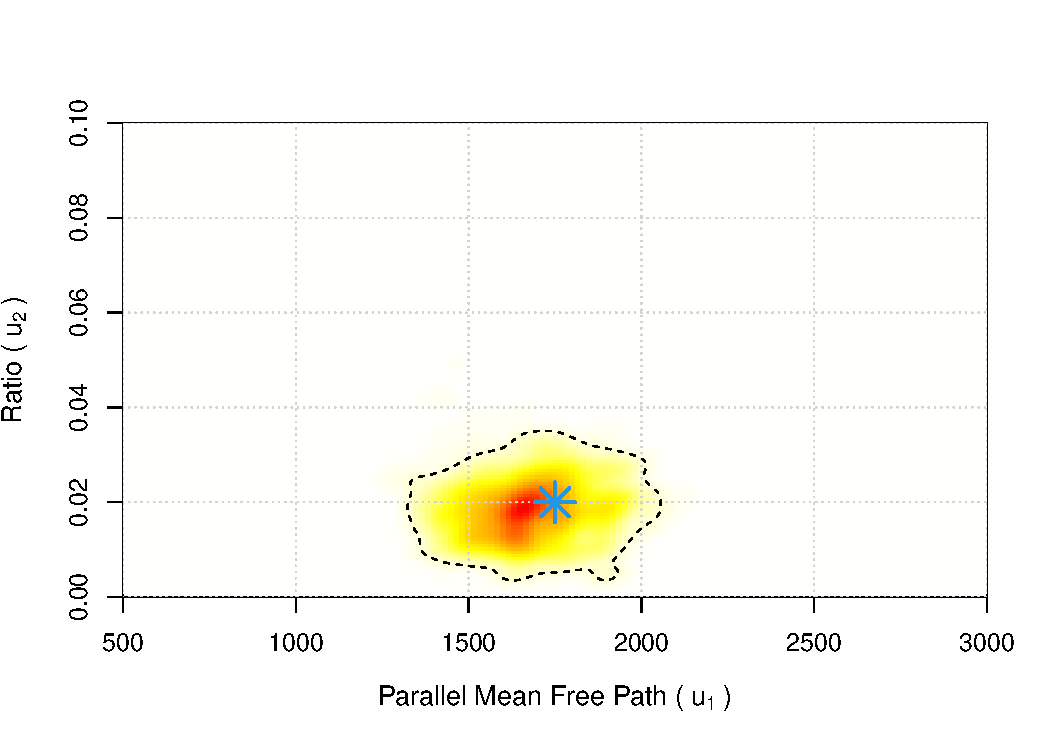
\includegraphics[scale=0.51,trim=0 15 15 45,clip=TRUE]{ibex_post_est.pdf}
\caption{Rough estimate of ENA rate
(counts/seconds) based on synthetic Poisson draws from a ``true'' computer
model setting and varying exposure times (top left). IBEX simulator output of
ENA rate at \textit{parallel mean free path} $= 1750$ and \textit{ratio} $=
0.02$ (top right). Predicted output via a fitted Scaled Vecchia surrogate at
estimated calibration parameters (bottom left). Posterior distribution of sampled model parameters $u$ (bottom right).
\label{f:ibex_synth_ex}}
\end{figure}

We run Algorithm \ref{alg:gibbs}, treating this synthetic data as $(X^F, Y^F)$
and using the provided computer model output (omitting responses for $u^*$) as
$(X^M, \lambda^M)$. We execute 10,000 MCMC iterations, throwing away 1,000 as
burnin and thin by 10. Figure \ref{f:ibex_synth_ex} displays the remaining
posterior samples of $u$ (bottom right) and a 95\% highest posterior density
(HPD) interval. The posterior mean of $u \mid Y^F$ lies near $u^*$,
demonstrating that our framework is able to concentrate mass around the true
model parameter. As a sanity check, we take posterior mean and plug it in to
our fitted Scaled Vecchia GP surrogate. The predicted output is shown in the
bottom left panel of Figure \ref{f:ibex_synth_ex}. There are some subtle
differences between the estimated sky map and the true $\lambda^*$ (i.e, the
shape and intensity of the ribbon vary slightly between the two). However, each
map could have reasonably generated the data we ``observe'' in the top left
panel.

\begin{figure}[ht!]
\centering
\includegraphics[scale=1.0,trim=0 0 0 0,clip=TRUE]{sim_bayes_inv_res.pdf}
\caption{Posterior distributions $u \mid Y^F$ and 95\% HPD intervals runs of
our Poisson Bayesian inverse problems framework on 36 different synthetic
datasets. Blue stars indicate the value $u^*$ from which the data was
simulated.
\label{f:synth_estimates_all}}
\end{figure}

To further validate our methodology, we apply this method to each unique model
parameter available. We have access to $n=66$ simulator runs, representing all
combinations for 11 unique values of parallel mean free path and 6 unique
values of ratio. The spread of parameter values is determined by space
scientists to include all values considered reasonable: parallel mean free path
ranges from 500-3000 astronomical units (AU); ratio values are unitless, and
span from 0.001 to 0.1. Due to the inability for the model to furnish posterior
samples beyond the boundary parameters, we do not test those combinations for
which at least one parameter is on its edge (i.e, when parallel mean free path
$\in \{500, 3000\}$ and/or ratio $\in \{0.001, 0.1\}$). Removing these edge
cases results in 36 remaining test runs. For each combination, we follow the
same procedure as above: select one model parameter $u$ and create simulated
observed satellite data, fit a  Scaled Vecchia surrogate on training data
excluding $u^*$, and run Algorithm \ref{alg:gibbs} to sample from the posterior
$u \mid Y^F$. Results are shown in Figure \ref{f:synth_estimates_all}.

Each panel shows posterior samples of $u \mid Y^F$ for a unique $u^*$. We have
indicated each $u^*$ that generated synthetic $Y^F$ as a blue star. Our 95\%
HPD intervals encompass the truth in 34 of the 36 of the iterations, near the
nominal coverage rate we'd expect. Therefore, we can confidently assert that
our proposed framework is able to recover the true parameter values from
synthetic satellite data. Next, we apply this to real data, with the goal of
helping scientists better understand the behavior of the heliosphere by
estimating these parameters for actual ENA counts collected by the IBEX
satellite.

%%%%%%%%%%%%%%%%%%%%%%%%%%%%%%%%%%%%%%%%%%%%%%%%%%%%%%%%%%%%%%%%%%%%%%%%%%%%%%%

% SECTION 5: IBEX Satellite Data
\section{IBEX Satellite Data}
\label{sec:ibex_real}

Space scientists at LANL have provided us with 14 years of data collected by
the IBEX satellite. IBEX is able to view the entire sky over a period of six
months through a series of regular adjustments. Therefore, dating back to 2008
we have access to $\sim$35 estimated \textit{sky maps}. The number of records
in each sky map varies across year, ranging from $\sim$8-15K observations. Each
row of the dataset contains the ENA origin location in Cartesian coordinates
($x$, $y$, $z$), time the satellite point{}ed at that location (in seconds),
counts of ENAs observed at one of six different energy levels (ESA), and a
background rate $\lambda_b$ (ENAs/sec).

ENAs are known to come from sources other than the heliosphere, so space
scientists quantify this noise and add it as a background rate that must be
accounted for. Although this rate is an estimate rather than an exact value, we
follow the lead of other researchers \citep{osthustheseus2023} and treat it as
constant in our work. For example, the left panel of Figure \ref{f:fig1}
displays ENA rates {\em after} the background rate has been substracted out.
For the purpose of solving the inverse problem, the mean in the Poisson
likelihood in Eq.~\ref{eq:pois_inv_bayes_mod} becomes $\lambda(X^F) = m(u, X^F)
- \lambda_{b}(X^F)$. We aim to pair the observed satellite data with the $n=66$
computer model runs to learn the distribution of IBEX simulator parameters
\textit{parallel mean free path} and \textit{ratio}.

%------------------------------------------------------------------------------
%% SECTION 5.1 - Heliospheric Computer Models
\subsection{Heliospheric Computer Models}
\label{sec:helio_comp_model}
%------------------------------------------------------------------------------

We have referred to the IBEX simulator throughout the entirety of this paper
without going into much detail. We focused on just two particular models
available among many, one for the GDF and one for the ribbon. We leave a more
in-depth physical interpretation and analysis of parameters to more appropriate
venues \citep{zirnstein2021dependence,zirnsteinGDFsims2015}, but to give some
context, we give a simple review here. The GDF model we use is constant and is
added on to the output of the ribbon simulator. For the ribbon model, one can
think of parallel mean free path as the distance a hydrogen ion travels beyond
the heliopause before interacting with another particle, receiving an electron,
and becoming an ENA. The ratio parameter is the fraction of parallel mean free
path and another measure of distance, the perpendicular mean free path.

Real data brings some additional complications, in particular when comparing to
computer models. The makeup of heliosphere changes over time, largely due to
the variations in the solar wind that accompany the sun's 11 or 21-year cycle.
Physicists therefore must account for these changes through additional
parameters, or restricting the application of their models to a specific
timeframe. This is the case for the GDF model, which corresponds to 2009-2011,
the first few years of IBEX's mission. On the other hand, the ribbon model
takes the approach of averaging over the entire sun-cycle. We factor in this
variation by only comparing satellite data from the years 2009-2011 to
simulator runs.

%%%%%%%%%%%%%%%%%%%%%%%%%%%%%%%%%%%%%%%%%%%%%%%%%%%%%%%%%%%%%%%%%%%%%%%%%%%%%%%

%------------------------------------------------------------------------------
%% SECTION 5.2 - Estimating parameters for real data
\subsection{Estimating parameters for real data}
\label{sec:ibex_exp}
%------------------------------------------------------------------------------

%% EXPERIMENT
%% - Explain set up of the experiment
%% - Show results from the real data
%% - Comment on the missalignment between simulator and reality

similar to that in Section \ref{sec:synth_data}, only
substituting in real data for simulated data. Therefore, we execute Algorithm
\ref{alg:gibbs} by initially fitting a Scaled Vecchia GP surrogate to all
$n=66$ computer model runs. Then, MCMC samples from the posterior distribution
of our model parameters, evaluating the likelihood of the real data given the
surrogate predictions at new proposed parameter values. Some things of note
are that we only use satellite data collected during the years 2011-2013. This
comes recommended by the space scientists, as the models are developed to
reflect the behavior of the Sun and corresponding solar wind during that time
period. Additionally, we only use ENAs collected at energy level ESA 4. This
energy level allows the best context for analysis, whereas lower ESAs have a
much weaker signal and higher ENAs overwhelm the analysis.

Results are shown in Figure \ref{f:real_estimates_all}.

\begin{figure}[ht!]
\centering
\includegraphics[scale=1.0,trim=0 0 0 0,clip=TRUE]{real_bayes_inv_res.pdf}
\caption{Posterior distributions for estimated calibration parameters for each unique
combination of values that has been treated as a holdout set.
\label{f:real_estimates_all}}
\end{figure}

%------------------------------------------------------------------------------
%% SECTION 5.3 - DISCREPANCY
\subsection{Discrepancy}
\label{sec:ibex_discrep}
%------------------------------------------------------------------------------

%% DISCREPANCY
%% - Refer to KOH, Higdon, and their use of discrepancy
%% - Introduce simple scaling discrepancy (iniclude some equations)
%% - Refer to results in Appendix for simulated data where we discover the true scale
%% - Explain set up for IBEX calibration with discrepancy
%% - Show results
%% - Comment on complexity of discrepancy. Scale isn't sufficient.
%% - Perhaps a stationary GP is not even sufficient

%%%%%%%%%%%%%%%%%%%%%%%%%%%%%%%%%%%%%%%%%%%%%%%%%%%%%%%%%%%%%%%%%%%%%%%%%%%%%%%

%%%%%%%%%%%%%%%%%%%%%%%%%%%%%%%%%%%%%%%%%%%%%%%%%%%%%%%%%%%%%%%%%%%%%%%%%%%%%%%

% SECTION 6: Discussion
\section{Discussion}
\label{sec:discuss}

We have introduced an effective tool for solving inverse problems using
Bayesian methods where 1) data from a field experiment is not normally
distributed and 2) computer model output is extremely high-dimensional,
demanding an approximation for the Gaussian process surrogate. In simulated
experiments, our framework provides accurate predictions at unsampled input
locations. Additionally, when provided with data where the underlying
calibration parameters are known, we can recover the truth at the nominal 95\%
rate. We applied this methodology to data collected from the IBEX satellite,
and corresponding simulator output generating heliospheric sky maps. When
faced with real data from the satellite, our method shows that large
discrepancies exist between the computer model and the physical process it
attempts to represent. Further collaboration is needed to inform the
theoretical astrophysicists responsible for model development where the model
is lacking, and improve its fidelity to the truth.

Our framework is only applied to counts assumed to come from a Poisson
distributed process. We encourage other practitioners to use this work in
other contexts where data from the field may come from some other distribution
(e.g. Negative Binomial, Bernoulli, Exponential, etc.). We recognize the
limitations of our method. First, the Scaled Vecchia GP surrogate for the
computer model fails to provide full uncertainty quantification on its
parameter estimates. A fully Bayesian framework could be developed, perhaps
with the use of a deep Gaussian process to handle the inherent
non-stationarity in the response surface. Finally, this project motivates the
need for a more exhaustive procedure to perform hypothesis testing for which
theoretical model is most probable, considering the data observed.

\subsection*{Acknowledgments}

RBG and SDB are grateful for funding from NSF CMMI 2152679. This work has been
approved for public release under LA-UR-XX-XXXX. SDB, DO and LJB were funded
by Laboratory Directed Research and Development (LDRD) Project 20220107DR.

\bibliography{ibex_bayes_inv}
\bibliographystyle{jasa}

\appendix

\end{document}
